\documentclass[11pt,a4paper]{article}

\usepackage[T1]{fontenc}
\usepackage[utf8]{inputenc}
\usepackage[provide=*,polish]{babel}
\usepackage{lmodern}
\usepackage[margin=2.4cm]{geometry}
\usepackage{amsmath,amssymb}
\usepackage{siunitx}
\usepackage{graphicx}
\usepackage{booktabs}
\usepackage{caption}
\usepackage{microtype}
\usepackage[hidelinks]{hyperref}

\sisetup{output-decimal-marker={,},per-mode=symbol,detect-all}
\captionsetup{font=small,labelfont=bf}

\title{\vspace{-1.5em}Walidacja prędkości detonacji w rurze uderzeniowej:\\
porównanie symulacji CFD z analizą termochemiczną (Cantera)}
\author{Antoni}
\date{\today}

\begin{document}
\maketitle

\begin{abstract}
\noindent
W~pracy przedstawiono walidację symulacji CFD detonacji wodorowo-powietrznej
w~rurze uderzeniowej z~klinem, inicjowanej przez ogniskowanie fali na~wierzchołku
klina (refleksja Macha). Prędkości fali padającej oraz detonacji wyznaczono
z~sygnałów ciśnienia w~sondach metodą czasu dotarcia (TOA), a~ich teoretyczne
odpowiedniki obliczono w~programie Cantera: stan za~falą uderzeniową
(model szoku zamrożonego) wraz z~prędkością gazu oraz prędkość detonacji
Chapmana--Jougueta (równowagowy Hugoniot). Uzyskano zgodność na~dwóch
niezależnych płaszczyznach: ciśnienie za~falą padającą ($\SI{2,54}{bar}$ wg~Cantery
vs.~$\approx\SI{2,5}{bar}$ z~CFD) oraz prędkość detonacji w~układzie laboratorium
($\SI{1261}{\meter\per\second}$ wg~teorii vs.~$\SIrange{1194}{1319}{\meter\per\second}$
z~CFD). Wykazano, że poprawne porównanie wymaga uwzględnienia prędkości gazu
za~falą padającą.
\end{abstract}

\section{Wprowadzenie i cel}
Celem pracy jest niezależna walidacja wyników symulacji CFD detonacji
w~rurze uderzeniowej, wykonanej solverem \texttt{ddtFoam} (OpenFOAM), poprzez
porównanie zmierzonych prędkości fal z~przewidywaniami klasycznej teorii
detonacji. Analizę termochemiczną przeprowadzono w~programie Cantera, co
pozwala oddzielić jakość modelu numerycznego od~efektów geometrycznych
i~uzyskać ilościową miarę poprawności rozwiązania.

Rozpatrywany przypadek dotyczy ubogiej mieszaniny wodoru z~powietrzem
($\SI{15}{\percent}$~mol.~$\mathrm{H_2}$, $\varphi\approx0{,}42$), w~której
fala uderzeniowa propaguje wzdłuż kanału ku klinowi, a~jej ogniskowanie
na~wierzchołku (refleksja Macha z~punktem potrójnym) prowadzi do~lokalnego
zapłonu i~uformowania się detonacji propagującej w~kierunku przeciwnym.

\section{Opis przypadku}
Mieszanina o~składzie molowym $\mathrm{H_2}:\mathrm{O_2}:\mathrm{N_2}
=0{,}15:0{,}1785:0{,}6715$ (15\% wodoru w~powietrzu) wypełnia kanał
o~ciśnieniu początkowym $P_0=\SI{1,024}{bar}$ i~temperaturze
$T_0=\SI{300}{\kelvin}$. Pole ciśnienia rejestrowano w~sondach
rozmieszczonych wzdłuż osi kanału ($y=\SI{0,0453}{\meter}$) oraz przy
wierzchołku klina. Współrzędne $x$ sond osiowych zestawiono
w~tabeli~\ref{tab:probes}.

\begin{table}[h]
\centering
\caption{Położenie sond osiowych wykorzystanych w~analizie TOA.}
\label{tab:probes}
\begin{tabular}{lcccccc}
\toprule
sonda & 1 & 2 & 3 & 4 & 5 & klin (6) \\
\midrule
$x$ [\si{\meter}] & 1,096 & 1,346 & 1,594 & 1,722 & 1,846 & 1,927 \\
\bottomrule
\end{tabular}
\end{table}

\section{Metodyka}

\subsection{Pomiar prędkości fal z~CFD (metoda TOA)}
Prędkość czoła fali wyznaczono z~różnicy czasów dotarcia (\emph{time of arrival})
do~kolejnych sond:
\begin{equation}
v=\frac{x_{i+1}-x_i}{t_{i+1}-t_i}.
\end{equation}
Dla \textbf{fali padającej} (propagującej w~kierunku $+x$) jako moment dotarcia
przyjęto pierwsze narastanie ciśnienia ponad poziom napełnienia
(sondy 2--5). Dla \textbf{detonacji} (kierunek $-x$, od~klina) wykorzystano
czas wystąpienia szczytu ciśnienia (sondy: klin$\to$5$\to$4). Rozdzielenie
obu zdarzeń jest konieczne, ponieważ każda sonda rejestruje je kolejno
w~czasie (rys.~\ref{fig:pt}).

\subsection{Model termochemiczny (Cantera)}
\paragraph{Fala padająca --- szok zamrożony.}
Stan za~falą uderzeniową wyznaczono z~równań zachowania masy, pędu i~energii
przy~zamrożonym składzie chemicznym:
\begin{equation}
\rho_1 u_1=\rho_2 u_2,\qquad
P_1+\rho_1 u_1^2=P_2+\rho_2 u_2^2,\qquad
h_1+\tfrac12 u_1^2=h_2+\tfrac12 u_2^2,
\end{equation}
gdzie $u_1=W$ jest prędkością fali. Liczbę Macha zdefiniowano jako
$M=W/a_1$, gdzie $a_1$ to~prędkość dźwięku w~niezaburzonej mieszaninie.
Prędkość gazu (\emph{particle velocity}) za~falą w~układzie laboratorium wynosi
\begin{equation}
u_p=u_1-u_2=W\!\left(1-\frac{\rho_1}{\rho_2}\right).
\label{eq:up}
\end{equation}

\paragraph{Detonacja Chapmana--Jougueta.}
Prędkość detonacji CJ obliczono jako minimum prędkości fali na~równowagowym
adiabacie Hugoniota. Dla zadanego stosunku objętości właściwych $v_2/v_1$
temperaturę produktów wyznaczano z~warunku Hugoniota
\begin{equation}
h_2-h_1=\tfrac12\,(P_2-P_1)(v_1+v_2),
\end{equation}
przy~równowagowym składzie produktów, a~odpowiadającą prędkość fali z~linii
Rayleigha
\begin{equation}
D=v_1\sqrt{\frac{P_2-P_1}{v_1-v_2}}.
\end{equation}
Warunek CJ odpowiada minimum $D$ względem $v_2/v_1$ (przepływ za~czołem osiąga
prędkość dźwięku). We~wszystkich obliczeniach zastosowano mechanizm
GRI-Mech~3.0.

\paragraph{Walidacja solvera.}
Dla mieszaniny stechiometrycznej $\mathrm{H_2}$--powietrze
($P=\SI{1}{atm}$, $T=\SI{300}{\kelvin}$) uzyskano
$D_{\mathrm{CJ}}=\SI{1969}{\meter\per\second}$,
$T_{\mathrm{CJ}}=\SI{2945}{\kelvin}$, $P_{\mathrm{CJ}}=\SI{15,7}{bar}$,
co~jest zgodne z~wartościami literaturowymi
($\approx\SI{1968}{\meter\per\second}$, $\approx\SI{2950}{\kelvin}$,
$\approx\SI{15,6}{bar}$). Potwierdza to~poprawność implementacji.

\section{Wyniki}

\subsection{Fala padająca}
Czasy dotarcia fali padającej do~kolejnych sond dają bardzo spójną prędkość:
\SI{564}{}, \SI{567}{} i~\SI{562}{\meter\per\second} na~kolejnych odcinkach
(rys.~\ref{fig:xt}). Wyniki analizy termochemicznej dla~$W=\SI{564}{\meter\per\second}$
zestawiono w~tabeli~\ref{tab:incident}.

\begin{table}[h]
\centering
\caption{Fala padająca: pomiar CFD oraz stan za~czołem wg~Cantery.}
\label{tab:incident}
\begin{tabular}{lcl}
\toprule
wielkość & wartość & źródło \\
\midrule
prędkość fali $W$ & \SI{564}{\meter\per\second} & CFD (TOA) \\
prędkość dźwięku $a_1$ & \SI{375}{\meter\per\second} & Cantera \\
liczba Macha $M$ & 1,50 & Cantera \\
ciśnienie za~czołem $P_2$ & \SI{2,54}{bar} & Cantera \\
temperatura za~czołem $T_2$ & \SI{397}{\kelvin} & Cantera \\
prędkość gazu $u_p$ & \SI{263}{\meter\per\second} & Cantera \\
\bottomrule
\end{tabular}
\end{table}

Obliczone ciśnienie za~falą ($P_2=\SI{2,54}{bar}$) pokrywa się z~poziomem
plateau rejestrowanym w~sondach~2 i~3 ($\approx\SI{2,5}{bar}$), co~stanowi
pierwszą, niezależną weryfikację zarówno pomiaru prędkości, jak i~modelu
termochemicznego.

\begin{figure}[h]
\centering
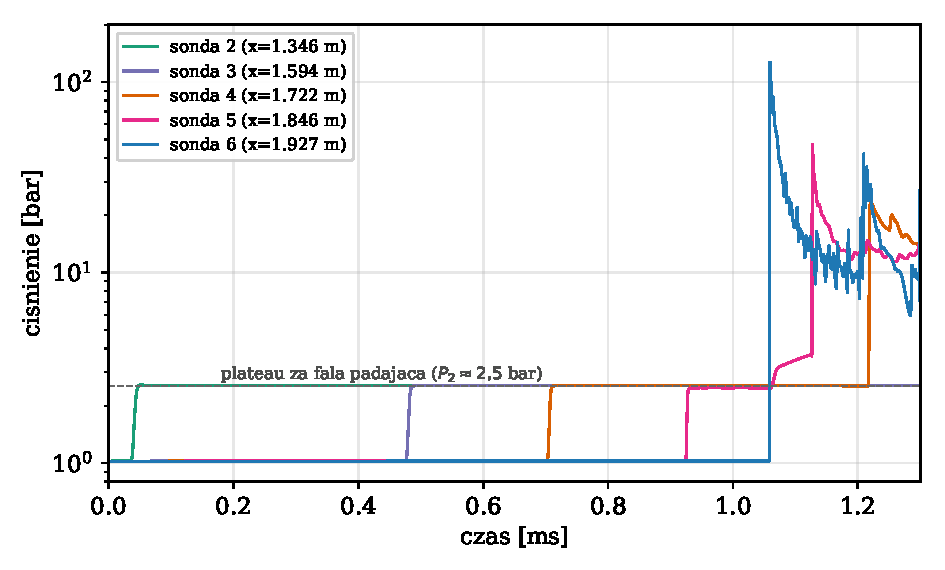
\includegraphics[width=0.82\linewidth]{fig_pt.pdf}
\caption{Przebiegi ciśnienia w~sondach (skala logarytmiczna). Widoczne plateau
za~falą padającą ($\approx\SI{2,5}{bar}$) oraz piki detonacji (sondy 4--6).
Detonacja zanika między sondą~4 a~3.}
\label{fig:pt}
\end{figure}

\subsection{Detonacja}
Detonacja inicjuje się przy~wierzchołku klina (piki ciśnienia
\SIrange{127}{237}{bar} w~sondach przyklinowych) i~propaguje w~kierunku $-x$.
Zmierzona prędkość wynosi \SI{1194}{\meter\per\second} na~odcinku klin$\to$5
(front jeszcze przesterowany po~inicjacji) oraz \SI{1319}{\meter\per\second}
na~odcinku 5$\to$4 (samopodtrzymująca się propagacja). Detonacja zanika
między sondą~4 a~3, co~jest typowe dla~ubogiej mieszaniny blisko granicy
detonowalności.

Detonacja propaguje w~gaz uprzednio sprężony i~wprawiony w~ruch przez~falę
padającą, dlatego prędkość CJ obliczono dla~stanu za~tą falą. Przejście
do~układu laboratorium wymaga odjęcia prędkości gazu (równ.~\ref{eq:up}):
\begin{equation}
D_{\mathrm{lab}}=D_{\mathrm{CJ}}-u_p.
\end{equation}
Zestawienie zawiera tabela~\ref{tab:det}.

\begin{table}[h]
\centering
\caption{Detonacja: pomiar CFD oraz wartości teoretyczne (Cantera).}
\label{tab:det}
\begin{tabular}{lcl}
\toprule
wielkość & wartość & źródło \\
\midrule
$D$ (klin$\to$5) & \SI{1194}{\meter\per\second} & CFD (TOA) \\
$D$ (5$\to$4) & \SI{1319}{\meter\per\second} & CFD (TOA) \\
$D_{\mathrm{CJ}}$ (stan napełnienia) & \SI{1516}{\meter\per\second} & Cantera \\
$D_{\mathrm{CJ}}$ (gaz sprężony) & \SI{1525}{\meter\per\second} & Cantera \\
$u_p$ (poprawka) & \SI{263}{\meter\per\second} & Cantera \\
$D_{\mathrm{lab}}=D_{\mathrm{CJ}}-u_p$ & \SI{1261}{\meter\per\second} & Cantera \\
\bottomrule
\end{tabular}
\end{table}

\begin{figure}[h]
\centering
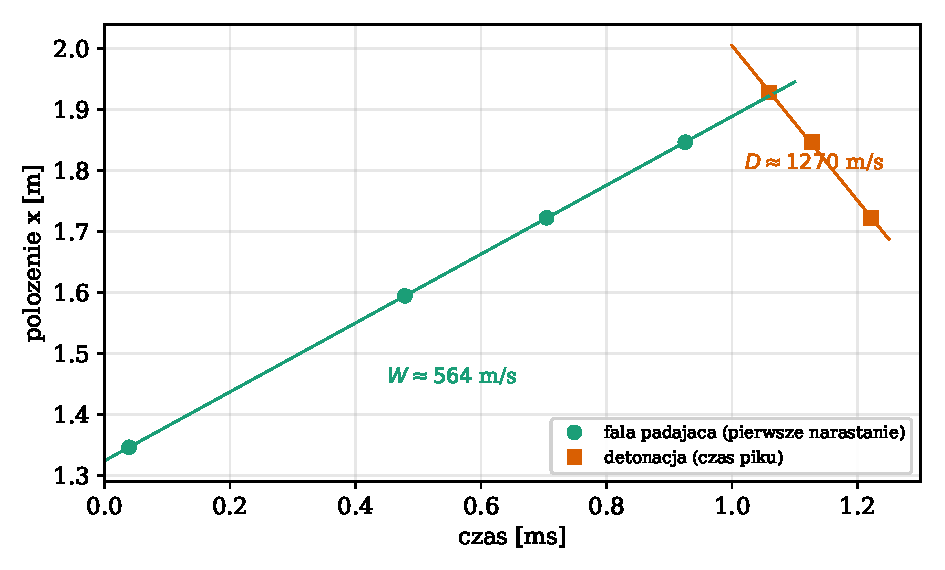
\includegraphics[width=0.82\linewidth]{fig_xt.pdf}
\caption{Diagram $x$--$t$ czoł fal. Nachylenie prostych odpowiada prędkościom
propagacji: fala padająca w~kierunku $+x$, detonacja w~kierunku $-x$.}
\label{fig:xt}
\end{figure}

\section{Dyskusja}
Teoretyczna prędkość detonacji w~układzie laboratorium
($\SI{1261}{\meter\per\second}$) bardzo dobrze zgadza się z~pomiarem CFD
(\SIrange{1194}{1319}{\meter\per\second}, średnio
$\approx\SI{1257}{\meter\per\second}$), co~potwierdza, że~front jest
w~przybliżeniu samopodtrzymujący się (zbliżony do~CJ).

Kluczowe jest uwzględnienie prędkości gazu. Porównanie samej prędkości CJ
($D_{\mathrm{CJ}}=\SI{1516}{\meter\per\second}$) z~wartością zmierzoną
dałoby pozorną rozbieżność rzędu \SI{20}{\percent}. Dopiero odjęcie
prędkości gazu za~falą padającą ($u_p=\SI{263}{\meter\per\second}$),
wynikającej z~kierunkowej zgodności ruchu gazu i~przeciwnego kierunku
propagacji detonacji, domyka bilans. Pokazuje to, że~wielkością właściwą
do~bezpośredniego porównania z~pomiarem czoła nie jest sama prędkość fali,
lecz prędkość fali w~układzie ruchomego gazu.

Zanik detonacji między sondami~4 a~3, przy~jednoczesnej zdolności do~inicjacji
poprzez ogniskowanie na~klinie, jest spójny z~marginalnym charakterem
mieszaniny ($\varphi\approx0{,}42$): bez~wzmocnienia geometrycznego fala nie
podtrzymuje samodzielnej propagacji.

\section{Wnioski}
\begin{enumerate}
\item Implementację obliczeń detonacji CJ w~Canterze zwalidowano na~mieszaninie
stechiometrycznej (\SI{1969}{} vs.~\SI{1968}{\meter\per\second}).
\item Stan za~falą padającą obliczony w~Canterze ($P_2=\SI{2,54}{bar}$) jest
zgodny z~plateau ciśnienia z~CFD ($\approx\SI{2,5}{bar}$).
\item Zmierzona prędkość detonacji (\SIrange{1194}{1319}{\meter\per\second})
zgadza się z~wartością teoretyczną w~układzie laboratorium
($\SI{1261}{\meter\per\second}$) po~uwzględnieniu prędkości gazu.
\item Wyniki potwierdzają poprawność symulacji CFD oraz samopodtrzymujący się,
choć~marginalny, charakter detonacji w~rozpatrywanej mieszaninie.
\end{enumerate}

\paragraph{Uwaga.} Obliczenia przyjmują temperaturę napełnienia
$T_0=\SI{300}{\kelvin}$; ciśnienie $P_0=\SI{1,024}{bar}$ odczytano
bezpośrednio z~danych. Zmiana $T_0$ wpływa na~wszystkie wielkości pochodne.

\end{document}
